\chapter{Pure Data Patches}\label{ap:pd_patches}
\Todo{make the patches more readable and replace the pics}

\section{Filter Based Additive Synthesis}
\begin{figure}[H]
  \centering
    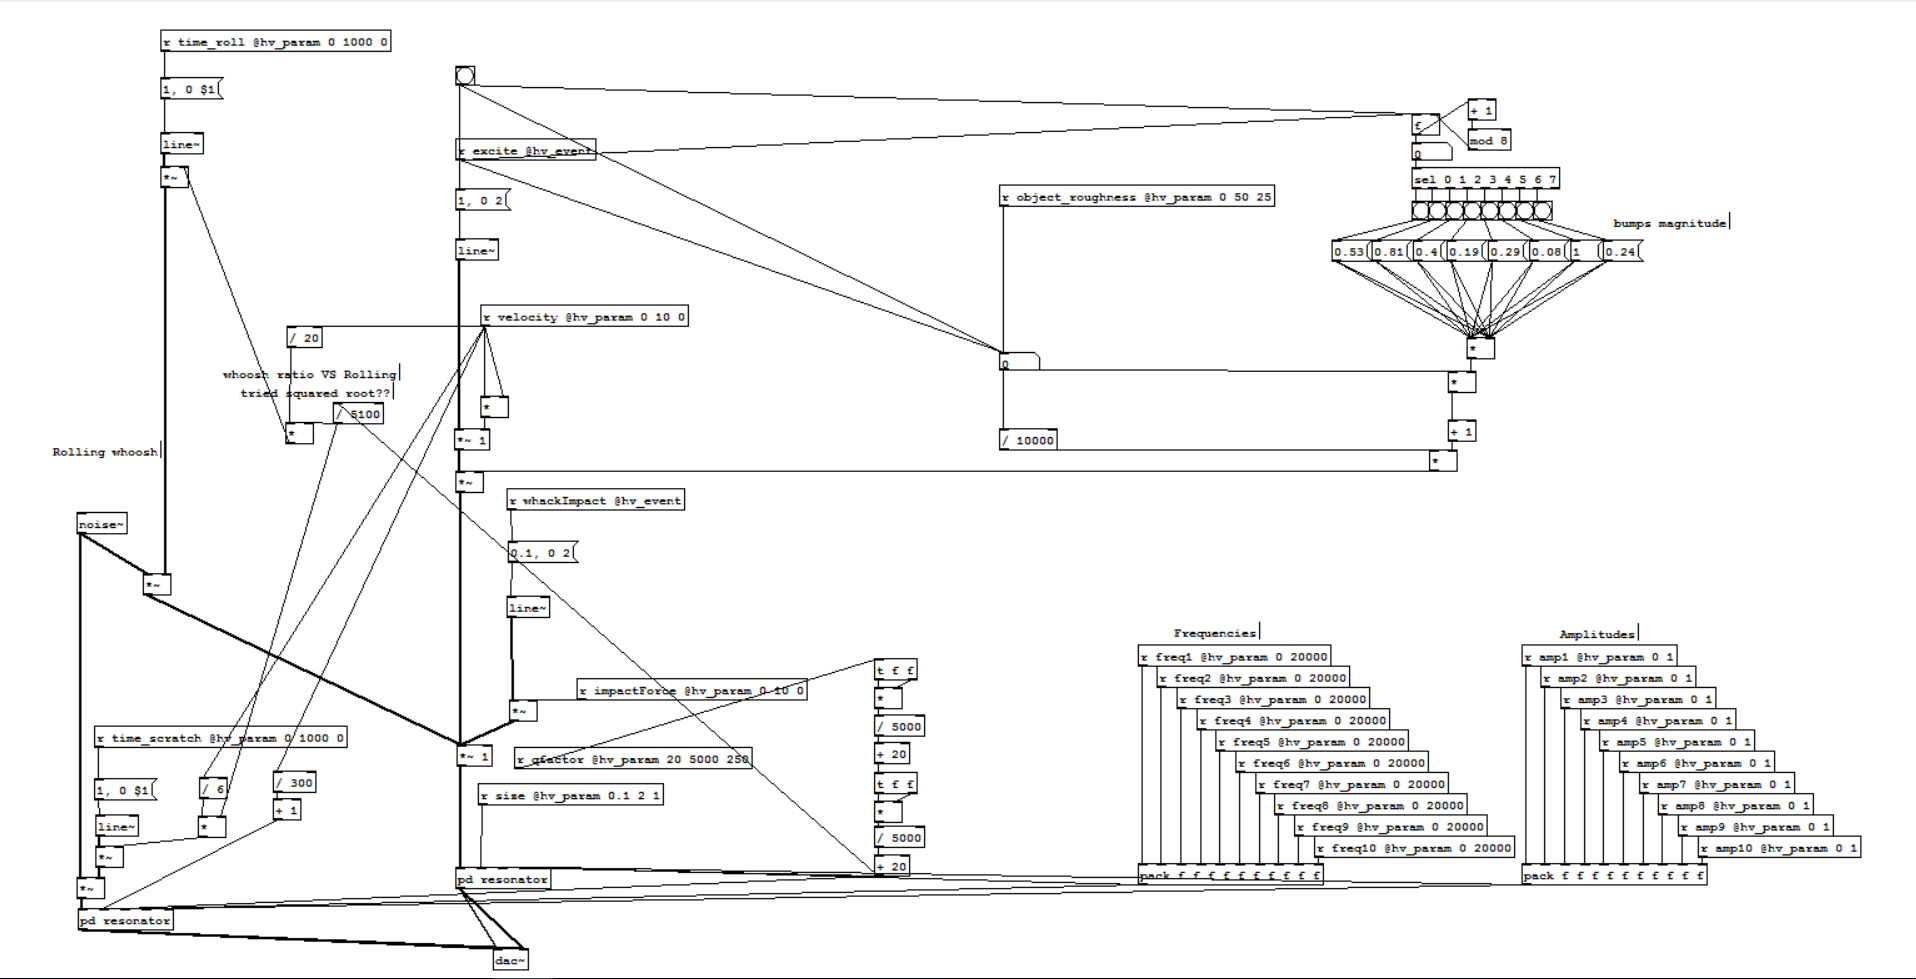
\includegraphics[width=\textwidth]{PdPatches/FBmain.PNG}
      \caption{The main Pure Data patch for the filter-based additive synthesis.}
      \label{fig:FBmain}
\end{figure}

\begin{figure}[H]
  \centering
    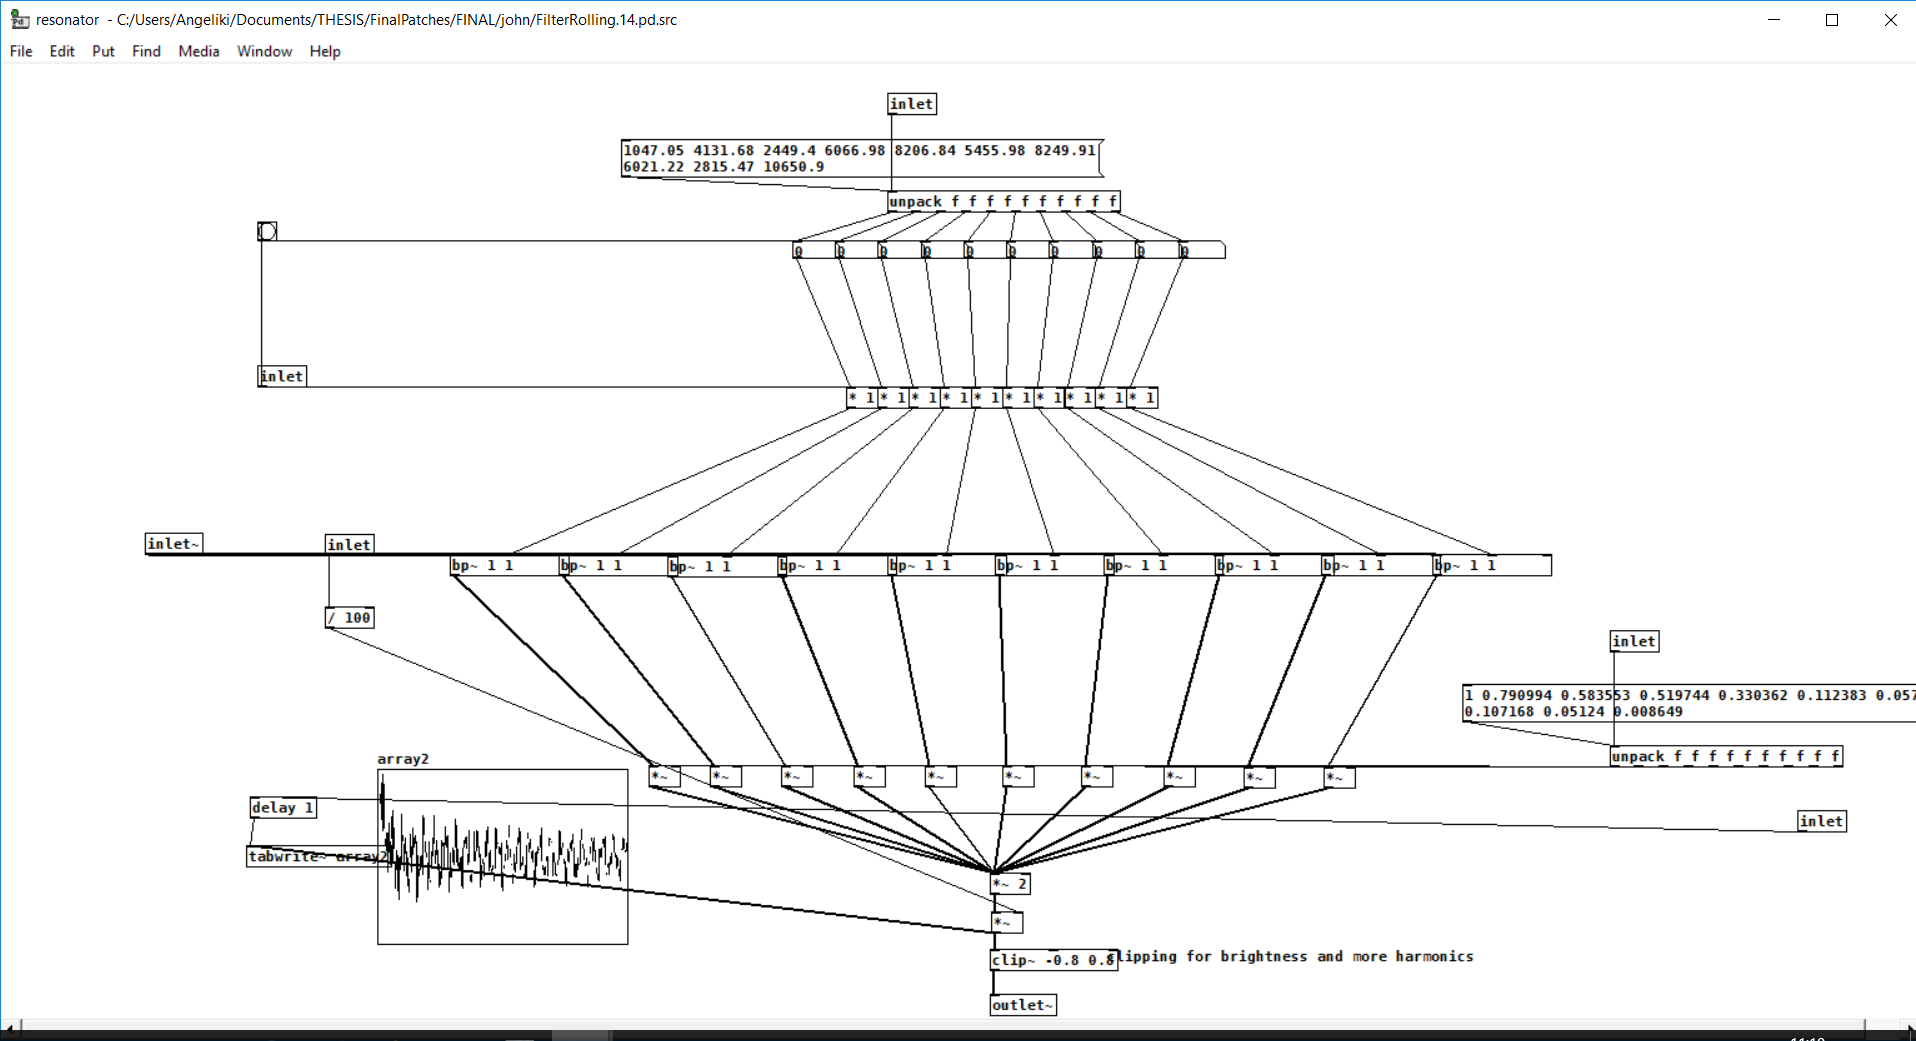
\includegraphics[width=\textwidth]{PdPatches/FBresonator.PNG}
      \caption{The resonator Pure Data patch for the filter-based additive synthesis.}
      \label{fig:FBres}
\end{figure}

\section{Sinusoidal Additive Synthesis}

\begin{figure}[H]
  \centering
    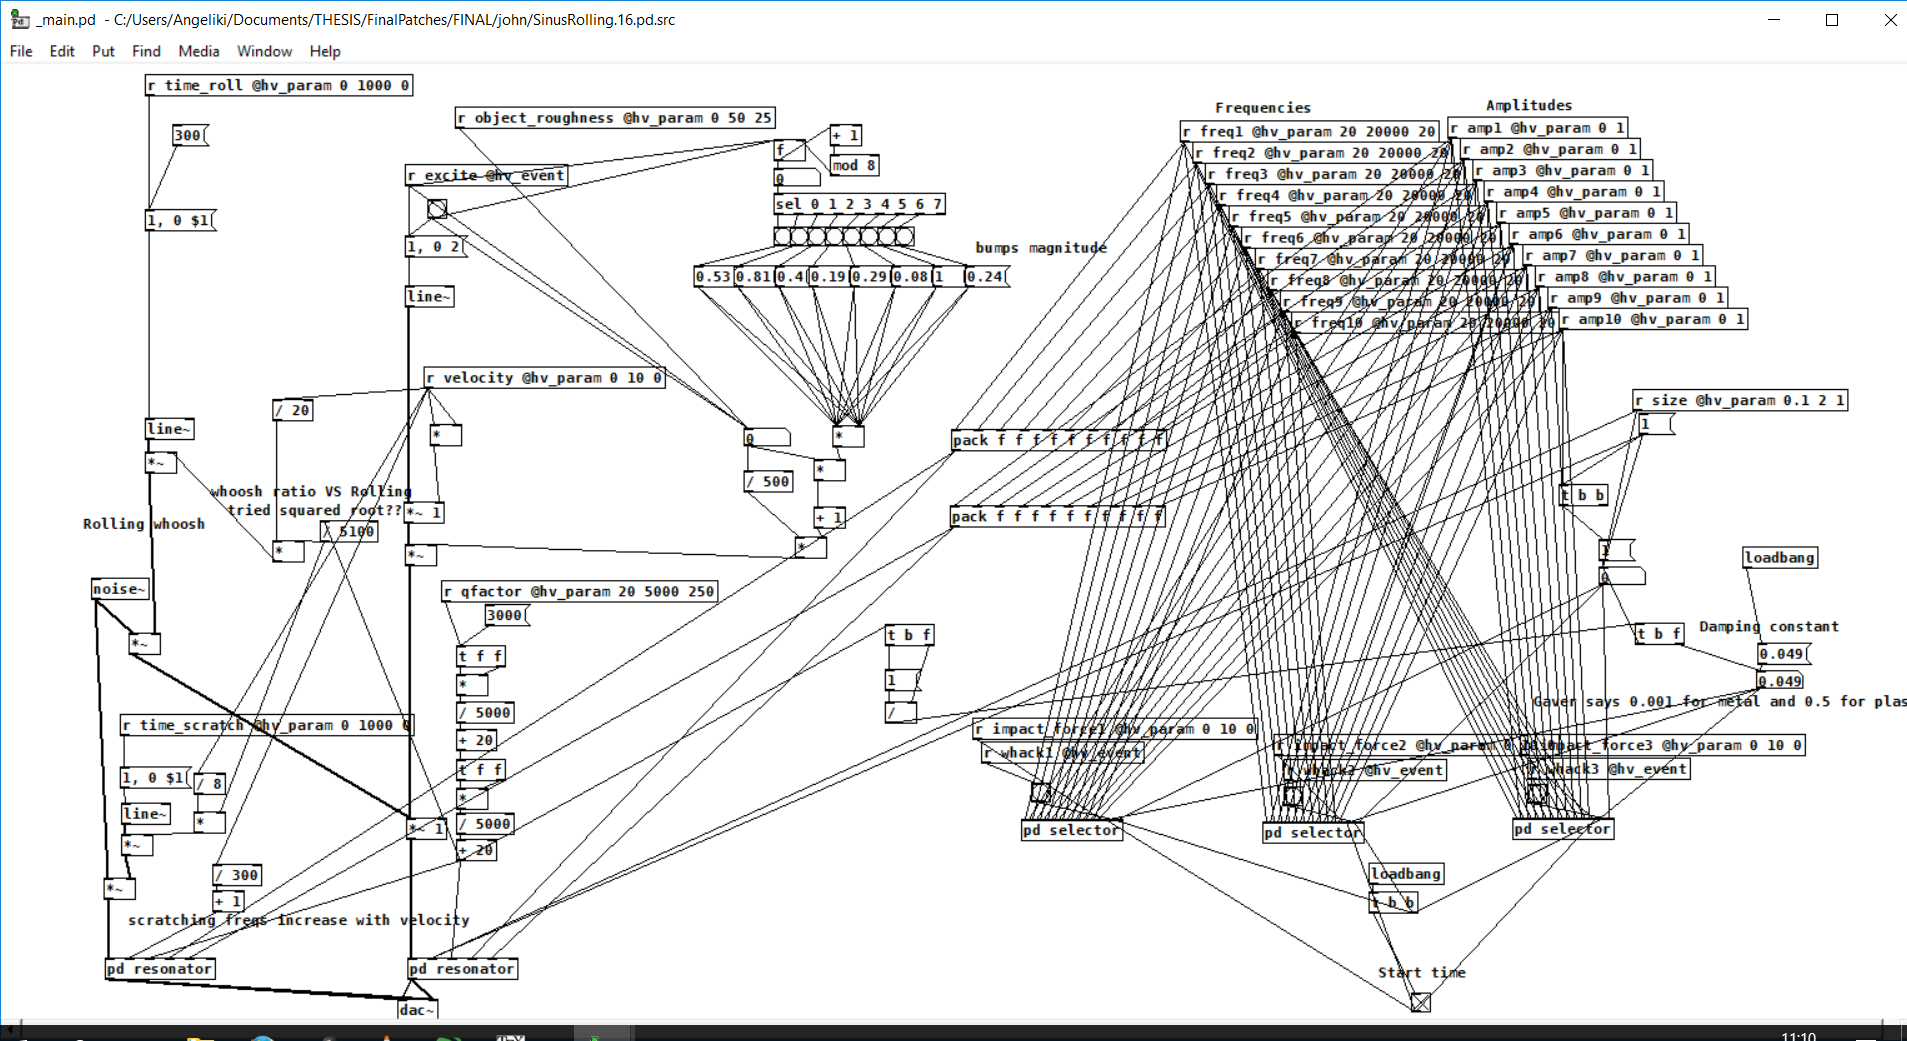
\includegraphics[width=\textwidth]{PdPatches/Smain.PNG}
      \caption{The main Pure Data patch for the sinusoidal additive synthesis.}
      \label{fig:Smain}
\end{figure}

\begin{figure}[H]
  \centering
    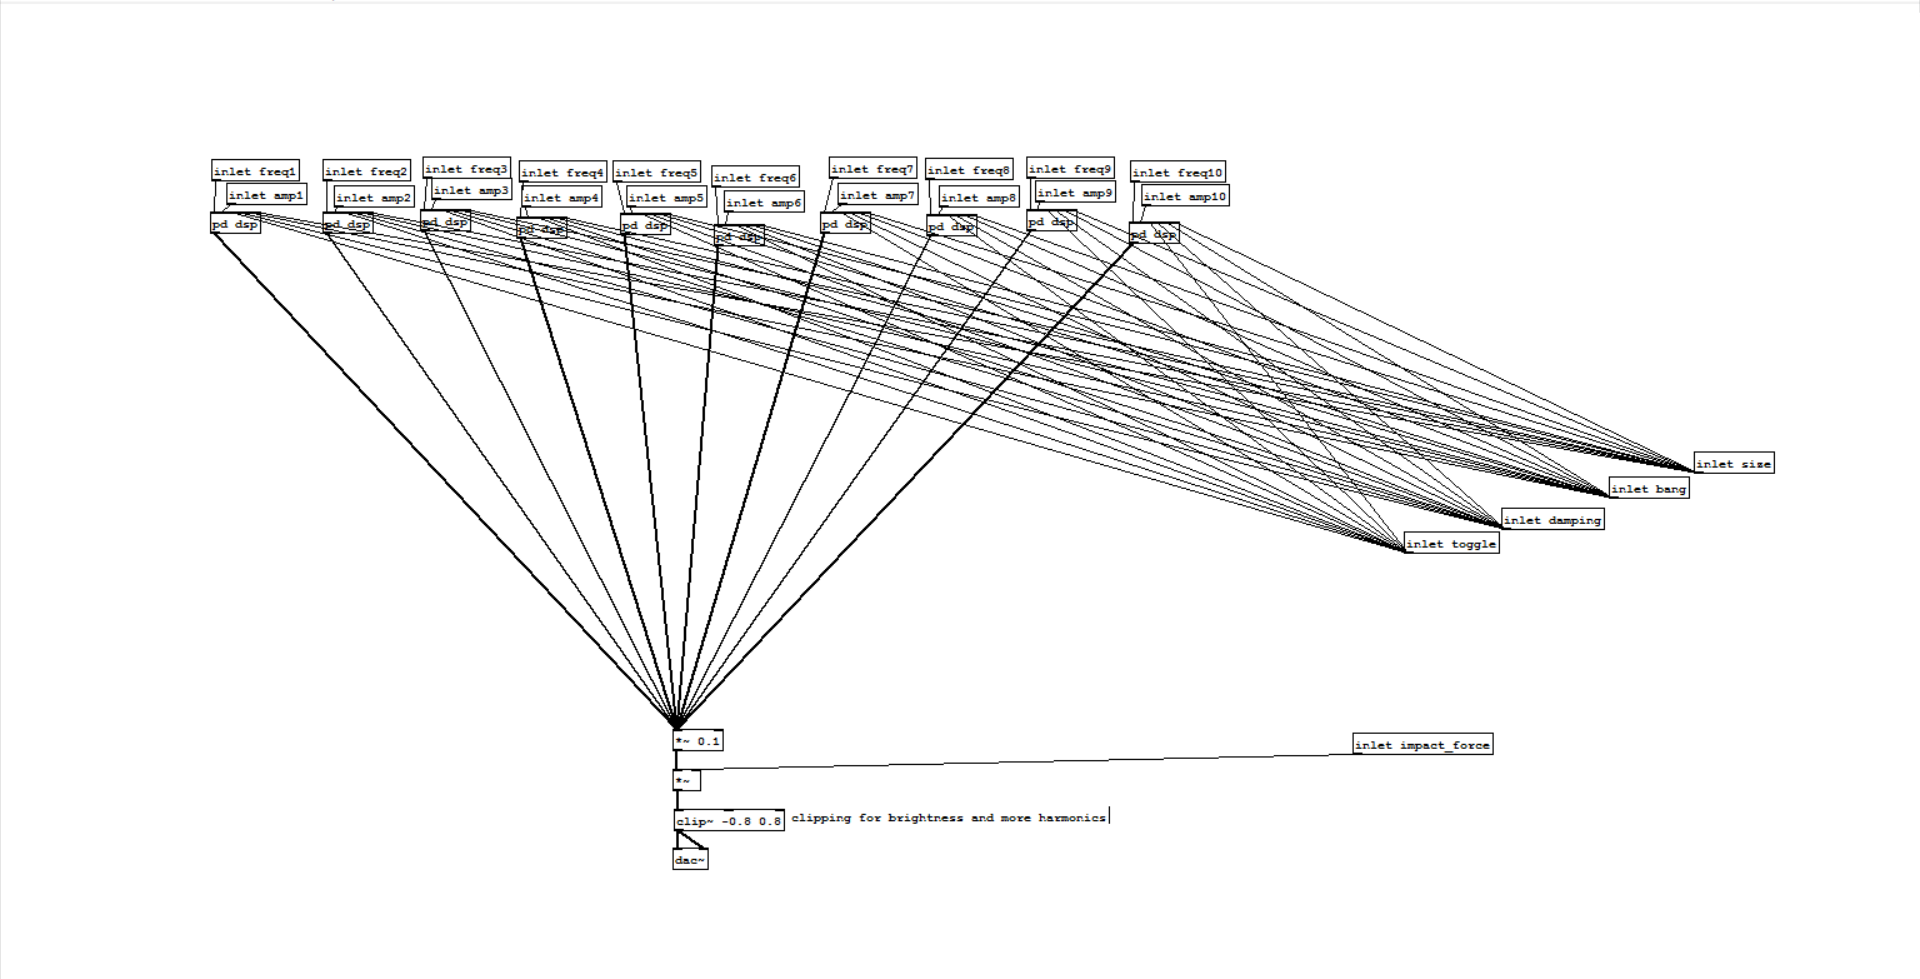
\includegraphics[width=\textwidth]{PdPatches/Sselector.PNG}
      \caption{The selector Pure Data patch for the filter-based additive synthesis.}
      \label{fig:Ssel}
\end{figure}

\begin{figure}[H]
  \centering
    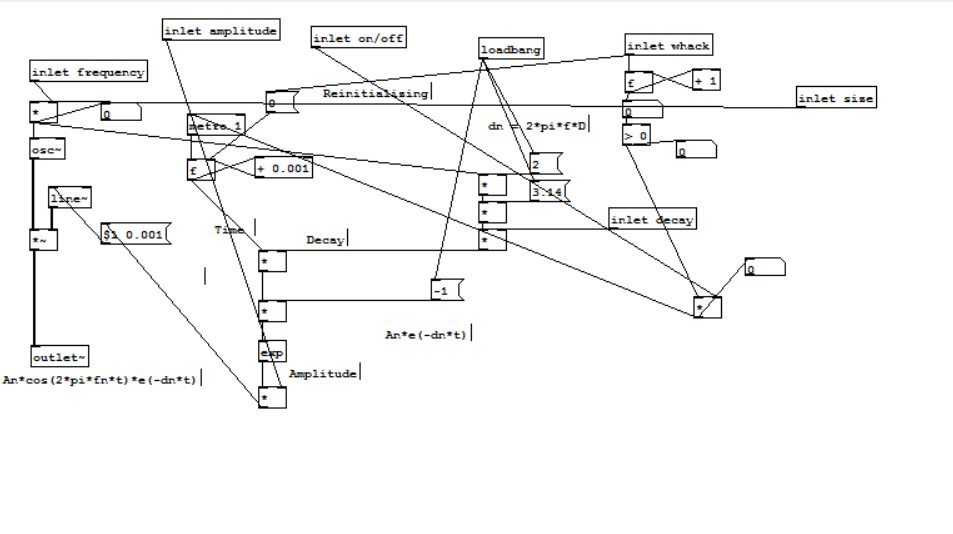
\includegraphics[width=\textwidth]{PdPatches/Sdsp.PNG}
      \caption{The dsp Pure Data patch for the filter-based additive synthesis.}
      \label{fig:Sdsp}
\end{figure}

\chapter{Interface of the Subjective Experiments}\label{ap:experiments}
The perceptual tests on people use the \textit{A-B} and \gls{MUSHRA} interface. Through instructions, participants were asked to choose the appropriate file for each test, fill the names of the tester and the test subject and choose a number of options, different for each part of the test (figure \ref{fig:exp_start}.

\begin{figure}[H]
  \centering
    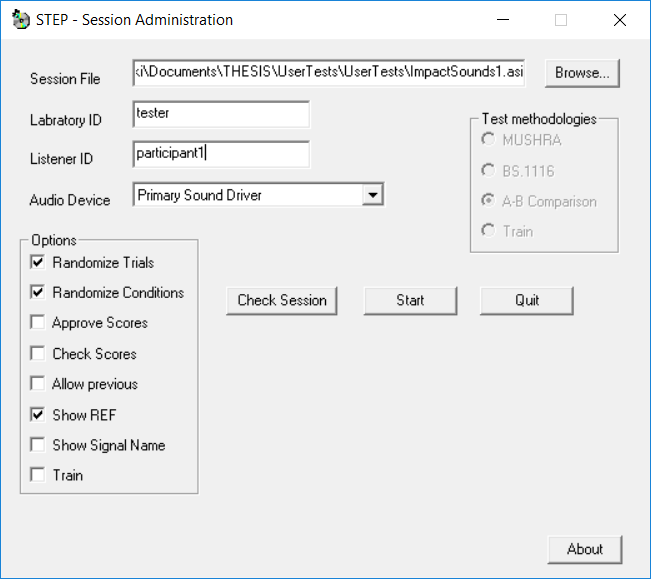
\includegraphics[width=0.8\textwidth]{test1_start.PNG}
        \caption{Settings interface.}
        \label{fig:exp_start}
\end{figure}

\section*{First Experiment}
The first experiment is an A-B test, where participants are encouraged to choose the closer to the reference between two sounds. All sounds are come from stuck objects and the reference sound is a real-world recording, while A-B options are synthesized sounds one for each synthesis method. It was split in two parts, to reduce the fatigue of participants. The options required for this part are the ``Randomize Trials'', which makes the trials show up in different order every time, the ``Randomize Conditions'', which randomizes the possibility an audio file to be assigned as an ``A'' or ``B'' option, and the ``Show REF'', which enables the reference sound button to appear. 

\begin{figure}[H]
    \centering  
     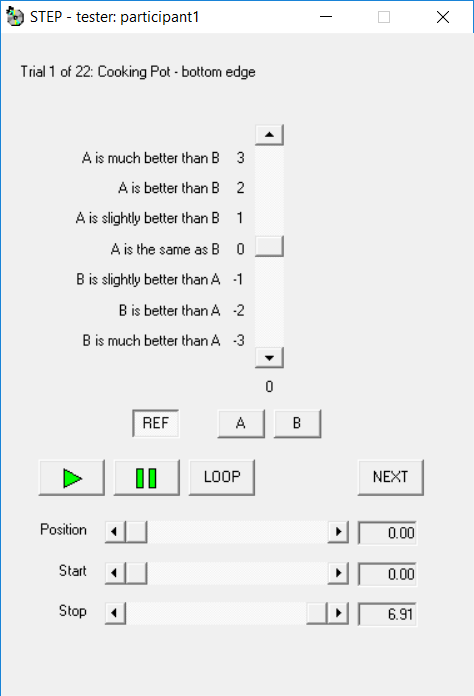
\includegraphics[width=0.7\textwidth]{test1_interface.PNG}
        \caption{The interface of the first experiment.}
        \label{fig:t1_ui}
\end{figure}

After pressing ``Start'', the window shown in figure \ref{fig:t1_ui} appears. Participants are prompted to press the ``Play'' button and the ``REF'', ``A'' and ``B'' buttons, each corresponding to one sound. They are, also, able to loop through the sounds instead of pressing ``Play'' every time they want to hear a sound again, or to shorten the sound length using the sliders on the bottom. 

After making up their mind, they are encouraged to position the vertical slider in the appropriate position and press ``NEXT'' to hear the next trial.

\section*{Second Experiment}
The second experiment is, also, an A-B test and is split in two parts; recordings and synthesized sounds. Participants listen to objects falling and colliding on inclining platforms with and without sound variation. The difference from the previous test is that there is no reference sound, since participants are asked to choose which sound they consider more qualitative. Hence, the option needed for this part are only the ``Randomize Trials'' and ``Randomize Conditions''.

\begin{figure}[H]
    \centering  
     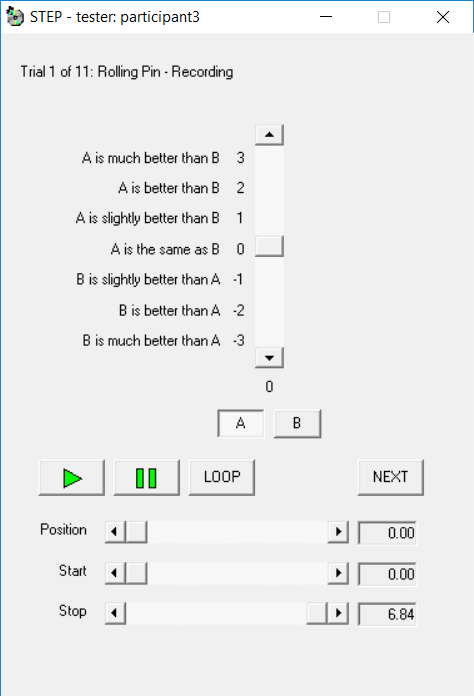
\includegraphics[width=0.7\textwidth]{test2_interface.PNG}
        \caption{The interface of the second experiment.}
        \label{fig:t2_ui}
\end{figure}

The interface of this test (figure \ref{fig:t2_ui} is similar to the previous one, except for the ``REF'' button. Participants were asked to follow the same procedure as before.

\section*{Third experiment}
The third experiment in a \gls{MUSHRA} test, where participants listen to ten different sounds produced by the same object falling on inclining platforms, while a range of different materials is assigned to it. The only option required for this part is ``Randomize Trials'', since the same increasing range of values for \gls{Q} is necessary. Participants are encouraged to listen the ten sounds and decide where a change in material happened. Then, they are asked to bring the corresponding slider down to zero.

\begin{figure}[H]
    \centering  
     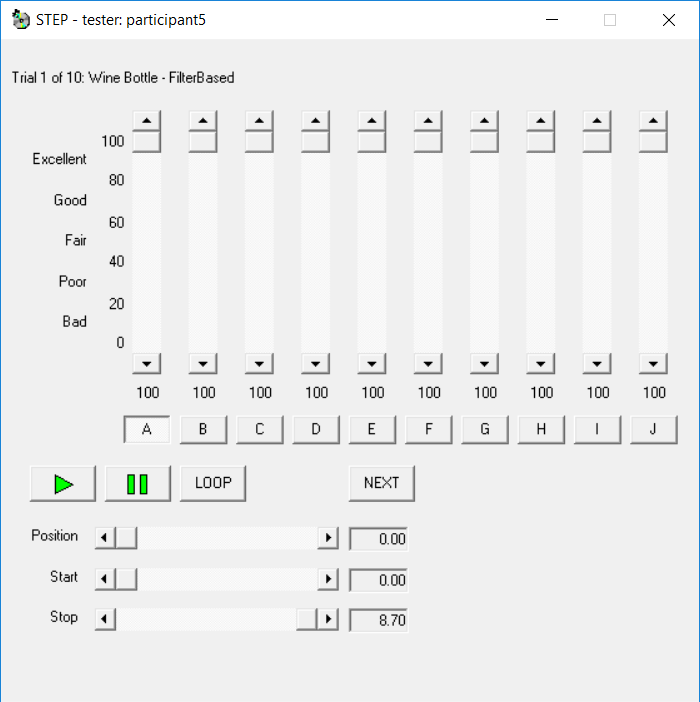
\includegraphics[width=0.8\textwidth]{test3_interface.PNG}
        \caption{The interface of the third experiment.}
        \label{fig:t3_ui}
\end{figure}

The interface of the third part of the experiment is displayed in figure \ref{fig:t3_ui}, where participants where asked to ignore the scaling of the slider and adjust it either at the top when no change in material was noticed, or at the bottom when it was noticed.

\chapter{Spectrograms}\label{ap:spectrograms}
Spectrograms of one object from each material used in this study. Each graph represents sound coming from one ``sound area'' of the object, either from the real-world recording or from the two synthesis methods (Sinusoidal Additive Synthesis and Filter-based Modal Synthesis).
\section*{Plastic bowl}

\begin{figure}[H]
  \centering
    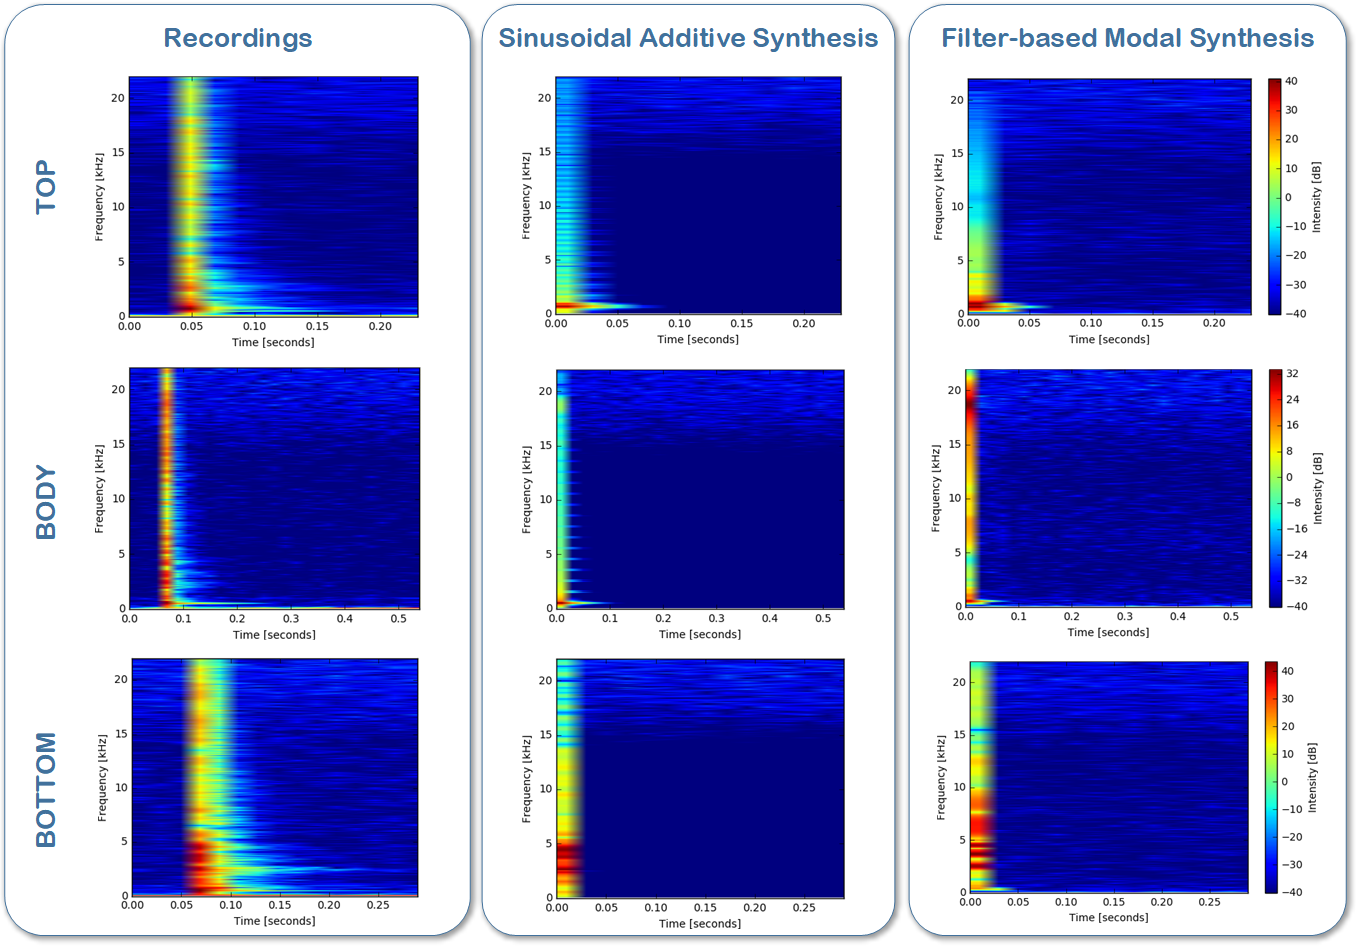
\includegraphics[width=\textwidth]{specs/bowl.png}
      \caption{Spectrograms of recordings and the two synthesis methods for the plastic bowl.}
      \label{fig:sp_bowl}
\end{figure}

\newpage

\section*{Wooden mortar}

\begin{figure}[H]
  \centering
    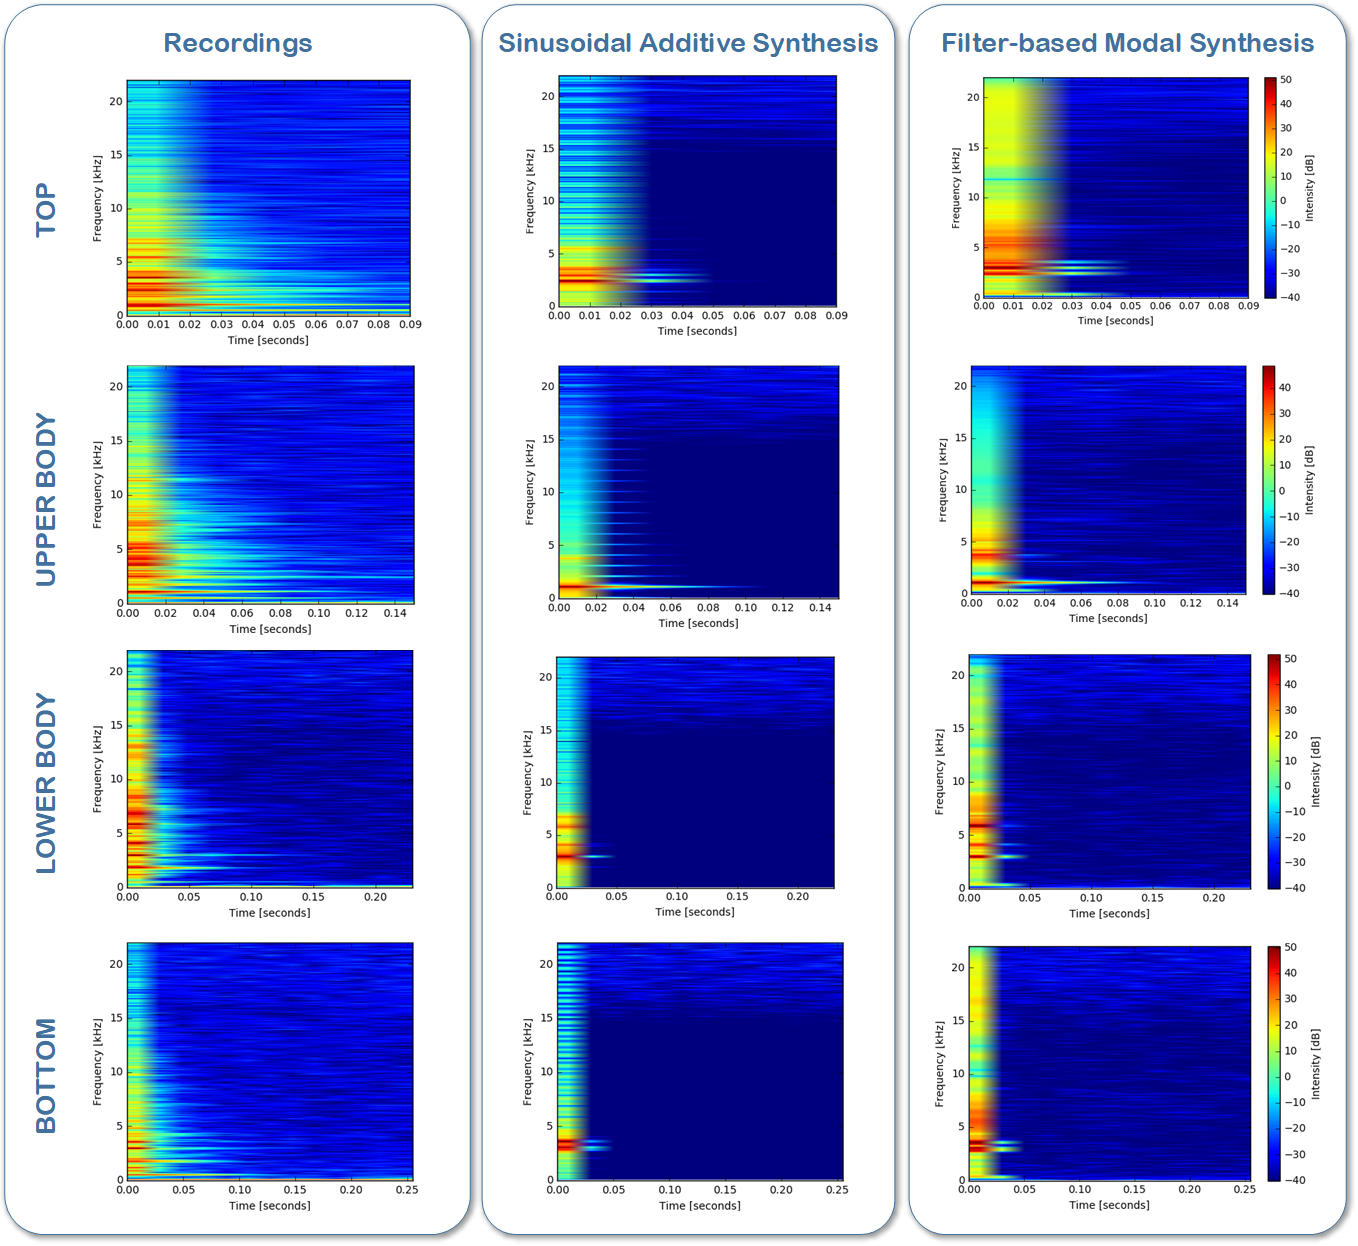
\includegraphics[width=\textwidth]{specs/mortar.png}
      \caption{Spectrograms of recordings and the two synthesis methods for the wooden mortar.}
      \label{fig:sp_mortar}
\end{figure}

\newpage

\section*{Ceramic plate}

\begin{figure}[H]
  \centering
    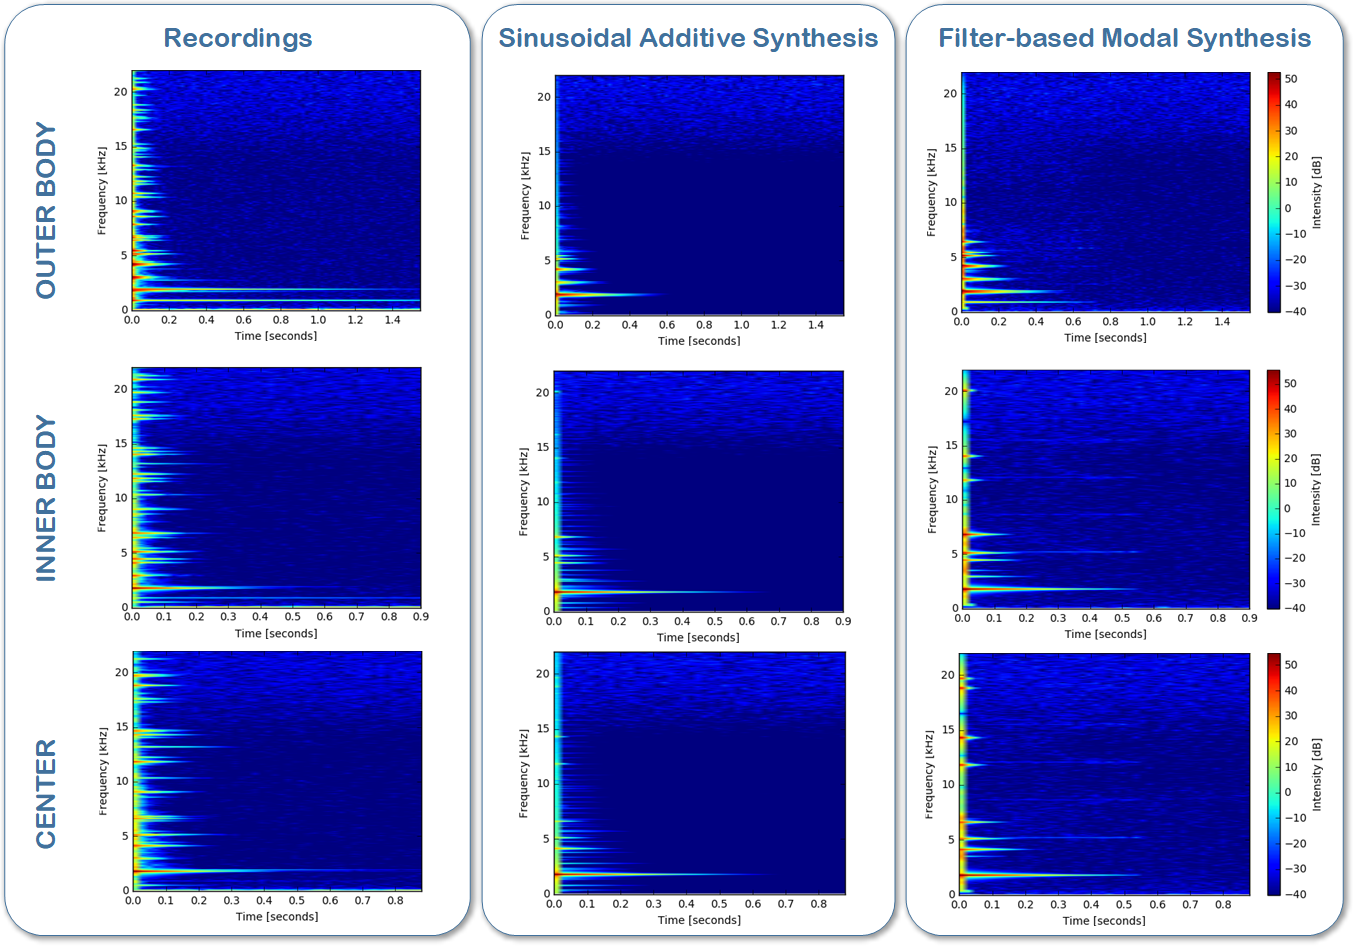
\includegraphics[width=\textwidth]{specs/plate.png}
      \caption{Spectrograms of recordings and the two synthesis methods for the ceramic plate.}
      \label{fig:sp_plate}
\end{figure}

\newpage

\section*{Wine glass}

\begin{figure}[H]
  \centering
    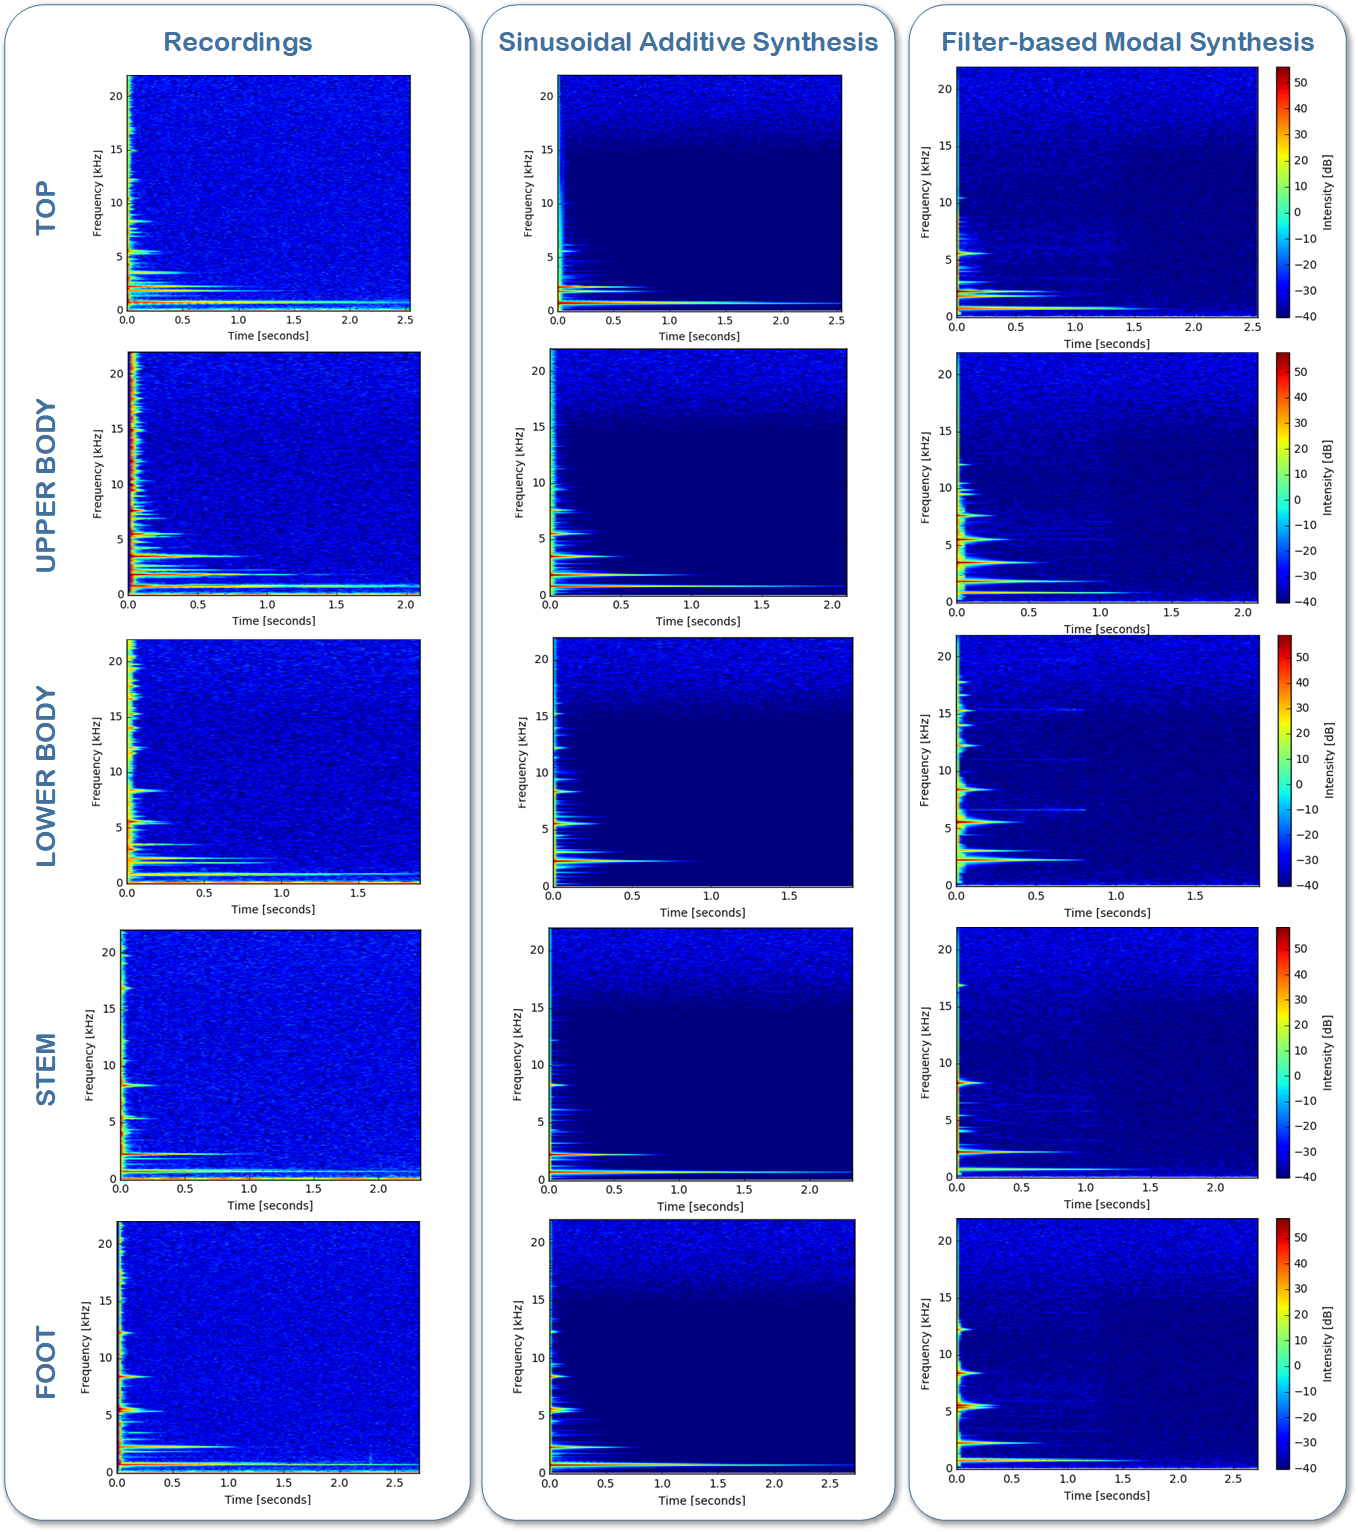
\includegraphics[width=\textwidth]{specs/glass.png}
      \caption{Spectrograms of recordings and the two synthesis methods for the wine glass.}
      \label{fig:sp_glass}
\end{figure}

\newpage

\section*{Metallic wok}

\begin{figure}[H]
  \centering
    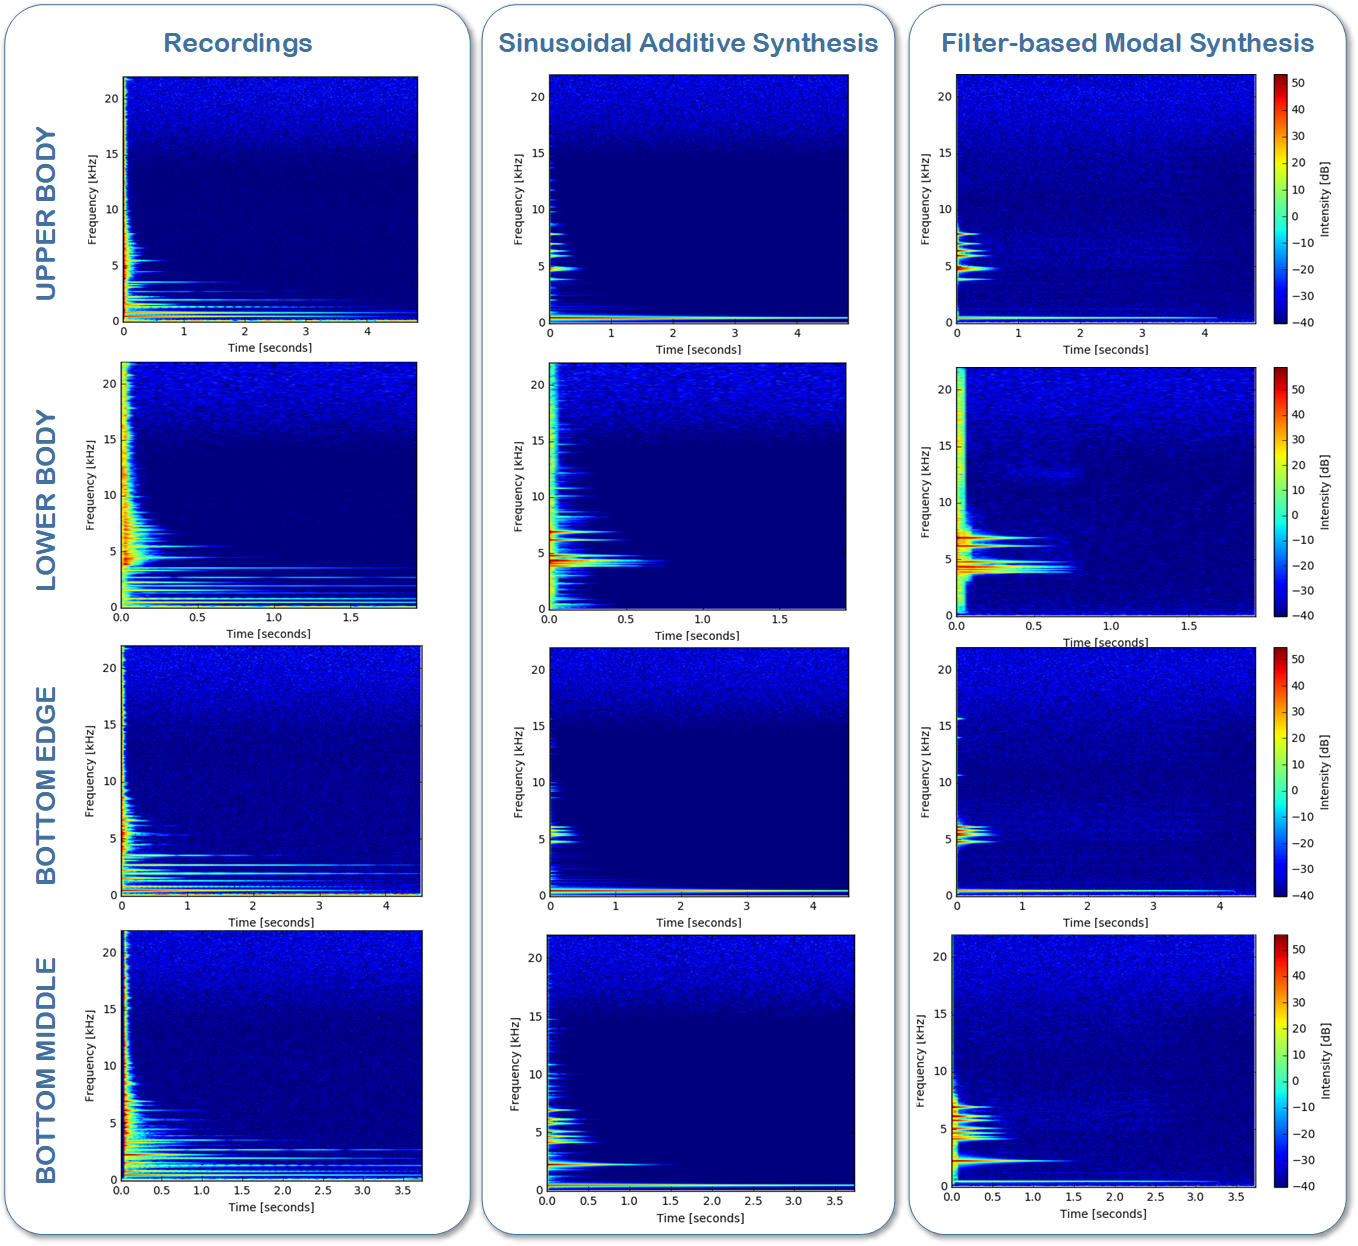
\includegraphics[width=\textwidth]{specs/wok.png}
      \caption{Spectrograms of recordings and the two synthesis methods for the metallic wok.}
      \label{fig:sp_wok}
\end{figure}

\chapter{User Guide for Tool Extension}\label{ap:guide}

%\begin{itemize}
%\item Decide on the areas to separate the object
%\item Record impact sounds
%\item Put audio files into the data extraction algorithm
%\item Measure object perimeter and weight of the object
%\item Put all data in Unity\textsuperscript{\textregistered} in Data Script
%\item Make a new item entry in Unity\textsuperscript{\textregistered}'s Audio Manager Script
%\item Make an FBX\textsuperscript{\textregistered} model of your object with the same dimensions and put it into a Unity\textsuperscript{\textregistered} scene as game object
%\item Assign the Audio Manager to the game object
%\item Tag the game object with the corresponding tag
%\item Adjust the material, size and object roughness sliders
%\end{itemize}

\begin{figure}[H]
  \centering
    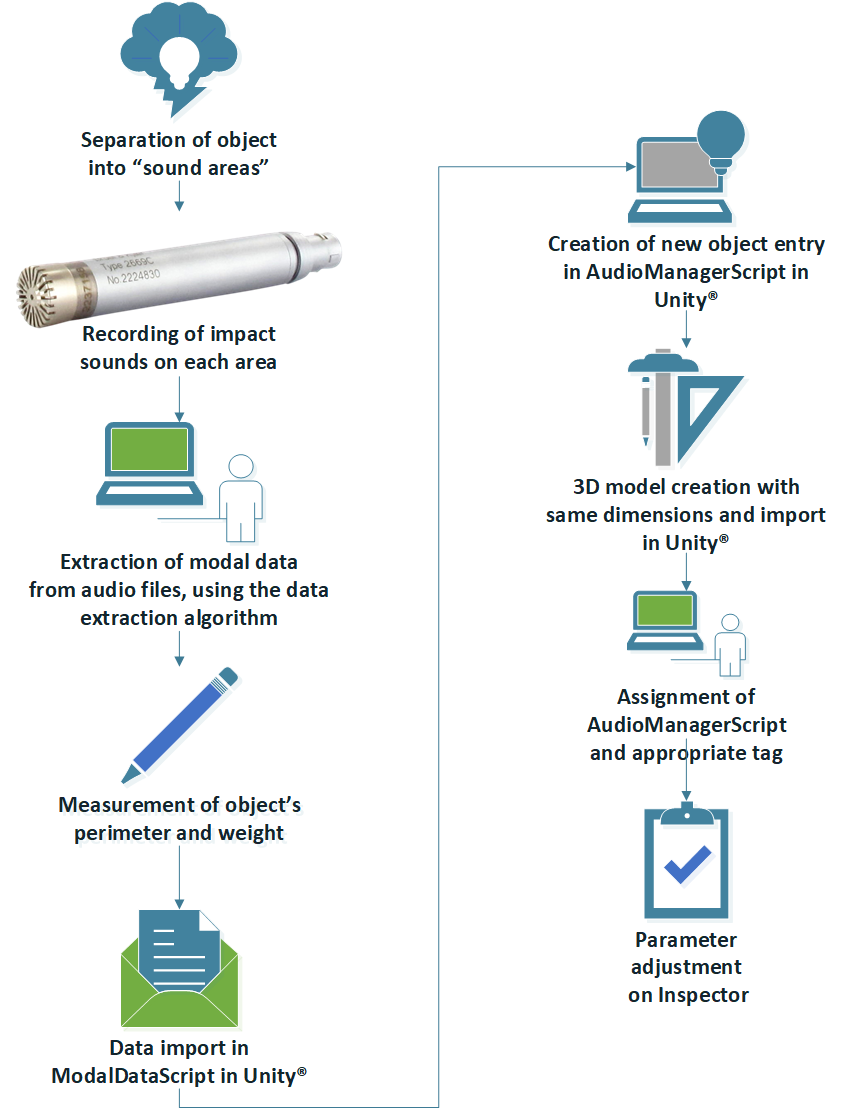
\includegraphics[width=0.7\textwidth]{Guide_images_line.png}
      \caption{Workflow for tool extension.}
      \label{fig:extension}
\end{figure}
